\documentclass[paper=letter,11pt]{scrartcl}

\KOMAoptions{headinclude=true, footinclude=false}
\KOMAoptions{DIV=14, BCOR=5mm}
\KOMAoptions{numbers=noendperiod}
\KOMAoptions{parskip=half}
\addtokomafont{disposition}{\rmfamily}
\addtokomafont{part}{\LARGE}
\addtokomafont{descriptionlabel}{\rmfamily}
%\setkomafont{pageheadfoot}{\normalsize\sffamily}
\setkomafont{pagehead}{\normalsize\rmfamily}
%\setkomafont{publishers}{\normalsize\rmfamily}
\setkomafont{caption}{\normalfont\small}
\setcapindent{0pt}
\deffootnote[1em]{1em}{1em}{\textsuperscript{\thefootnotemark}\ }


\usepackage{amsmath}
\usepackage[varg]{txfonts}
\usepackage[T1]{fontenc}
\usepackage{graphicx}
\usepackage{xcolor}
\usepackage[american]{babel}
% hyperref is needed in many places, so include it here
\usepackage{hyperref}

\usepackage{xspace}
\usepackage{multirow}
\usepackage{float}


\usepackage{braket}
\usepackage{bbm}
\usepackage{relsize}
\usepackage{tcolorbox}

\def\ketY{\ensuremath{\ket {\Psi}}}
\def\iGeV{\ensuremath{\textrm{GeV}^{-1}}}
%\def\mp{\ensuremath{m_{\textrm{proton}}}}
\def\rp{\ensuremath{r_{\textrm{proton}}}}
\def\me{\ensuremath{m_{\textrm{electron}}}}
\def\aG{\ensuremath{\alpha_G}}
\def\rAtom{\ensuremath{r_{\textrm{atom}}}}
\def\rNucl{\ensuremath{r_{\textrm{nucleus}}}}
\def\GN{\ensuremath{\textrm{G}_\textrm{N}}}
\def\ketX{\ensuremath{\ket{\vec{x}}}}
\def\ve{\ensuremath{\vec{\epsilon}}}


\def\ABCDMatrix{\ensuremath{\begin{pmatrix} A &  B  \\ C  & D \end{pmatrix}}}
\def\xyprime{\ensuremath{\begin{pmatrix} x' \\ y' \end{pmatrix}}}
\def\xyprimeT{\ensuremath{\begin{pmatrix} x' &  y' \end{pmatrix}}}
\def\xy{\ensuremath{\begin{pmatrix} x \\ y \end{pmatrix}}}
\def\xyT{\ensuremath{\begin{pmatrix} x & y \end{pmatrix}}}

\def\IMatrix{\ensuremath{\begin{pmatrix} 0 &  1  \\ -1  & 0 \end{pmatrix}}}
\def\IBoostMatrix{\ensuremath{\begin{pmatrix} 0 &  1  \\ 1  & 0 \end{pmatrix}}}
\def\JThree{\ensuremath{\begin{pmatrix}    0 & -i & 0  \\ i & 0  & 0 \\ 0 & 0 & 0 \end{pmatrix}}} 
\def\JTwo{\ensuremath{\begin{bmatrix}    0 & 0 & -i  \\ 0 & 0  & 0 \\ i & 0 & 0 \end{bmatrix}}}
\def\JOne{\ensuremath{\begin{bmatrix}    0 & 0 & 0  \\ 0 & 0  & -i \\ 0 & i & 0 \end{bmatrix}}}
\def\etamn{\ensuremath{\eta_{\mu\nu}}}
\def\Lmn{\ensuremath{\Lambda^\mu_\nu}}
\def\dmn{\ensuremath{\delta^\mu_\nu}}
\def\wmn{\ensuremath{\omega^\mu_\nu}}
\def\be{\begin{equation*}}
\def\ee{\end{equation*}}
\def\bea{\begin{eqnarray*}}
\def\eea{\end{eqnarray*}}
\def\bi{\begin{itemize}}
\def\ei{\end{itemize}}
\def\fmn{\ensuremath{F_{\mu\nu}}}
\def\fMN{\ensuremath{F^{\mu\nu}}}
\def\bc{\begin{center}}
\def\ec{\end{center}}
\def\nus{$\nu$s}

\def\adagger{\ensuremath{a_{p\sigma}^\dagger}}
\def\lineacross{\noindent\rule{\textwidth}{1pt}}

\newcommand{\multiline}[1] {
\begin{tabular} {|l}
#1
\end{tabular}
}

\newcommand{\multilineNoLine}[1] {
\begin{tabular} {l}
#1
\end{tabular}
}



\newcommand{\lineTwo}[2] {
\begin{tabular} {|l}
#1 \\
#2
\end{tabular}
}

\newcommand{\rmt}[1] {
\textrm{#1}
}


%
% Units
%
\def\m{\ensuremath{\rmt{m}}}
\def\GeV{\ensuremath{\rmt{GeV}}}
\def\pt{\ensuremath{p_\rmt{T}}}


\def\parity{\ensuremath{\mathcal{P}}}

\usepackage{cancel}
\usepackage{ mathrsfs }
\def\bigL{\ensuremath{\mathscr{L}}}

\usepackage{ dsfont }



\usepackage{fancyhdr}
\fancyhf{}

%\documentclass[margin,line]{res}
\usepackage{braket}

\def\ketY{\ensuremath{\ket {\Psi}}}
\def\iGeV{\ensuremath{\textrm{GeV}^{-1}}}
\def\mp{\ensuremath{m_{\textrm{proton}}}}
\def\me{\ensuremath{m_{\textrm{electron}}}}
\def\aG{\ensuremath{\alpha_G}}

\begin{document}

\textbf{\Huge Lecture 2}

\section{The right way to think about the world}

Talked last time about what our world consists of Matter/Forces ect.
This class we will start by talking about the ``right way'' to view all of this. 

Something that is not often taught (even in gradschool).
However it is easy and extremely powerful....

Compton lectures that I gave. 
Got into trouble. 
Diagrams like: 
Feature of Life -> Evolution -> DNA -> molecules -> chemistry  -> Atoms ->  Electrons-> Quantum Mechanics -> Standard Model
``Newton's Dream''

Go through a few examples of this kind of reasoning:
Teeth behind these statements

Idea that can describe world around us using a few basic physical parameters.
Powerful (Fun!) way of estimating $\sim$anything to order of magnitude.

\textbf{Dimensional Analysis and ``$\sim$''}

Put in the right physics to get answers to within ``geometric factors'':
\begin{itemize}
\item[-] Wont worry about factors of 2 or $\pi$ etc
\item[-] Use ``$\sim$'' not ``=''
\end{itemize}

\underline{Examples}

(Volume of something) $\sim$ (size$)^3$
Cube = $R^{3}$ $\sim$ $R^3$\\
Sphere = 4/3$\pi R^3$ = 4.2 R3 $\sim$ $R^3$\\
Sphere = 1/6$\pi D^3$  $\sim$ $D^3$\\
Cylinder = R$\times\pi R^{2}$  $\sim$ $R^3$  (if two scales use $r^2R$) 

Kinematic energy = 1/2 m$v^2$ $\sim$ m$v^2$\\
Ive been doing this already: ``$\Delta$p$\Delta X \geq $ h''
(...it is really $\Delta$p$\Delta X \geq $ h/(4$\pi$) )

\textbf{Natural Units}

Units...

I hate units! All numbers are really unit-less.
Always comparing some quantity relative to some standard. 
We will work in “Natural Units”.

Very easy. (Much easier than Metric/British/cgm/mks ...) \\
- Standard is set by basic physical principles.\\
- Numbers have direct physical interpretations.

c $\equiv$ 1: [Distance]/[Time] $\equiv$ 1\\
- Time and distance have same units\\
- Already familiar with this: ``Its about an hour from here''\\
- E = m\\

h $\equiv$ 1: [Energy]$\times$[Time] = 1 and [Energy]$\times$[Distance] = 1\\
- Energy (or Mass) is inversely related to distance or time.

Write everything in terms of [Energy]: Will often use 1 GeV $\sim$ \mp\ as basic unit.

Will now do everything in terms of GeV. 
Can use conversions to get back to human units

\textbf{Conversions:}\\
GeV = $10^-27 $ kg\\
\iGeV = $10^{-16}$ m\\
\iGeV = $6 \times 10^{-25}$ s\\

\underline{Examples:}\\
Proton Weight:  GeV \\
Proton Size:    \iGeV \\
My height: 1m $\sim$ 10$^{16}$ \iGeV \textit{(I am as tall as $10^{16}$ protons stacked on top of each other)}\\
My weight: 100kg $\sim$ 10$^{29}$ GeV \textit{(I am made of $10^{29}$ protons)}


\begin{figure}[h]
\centering
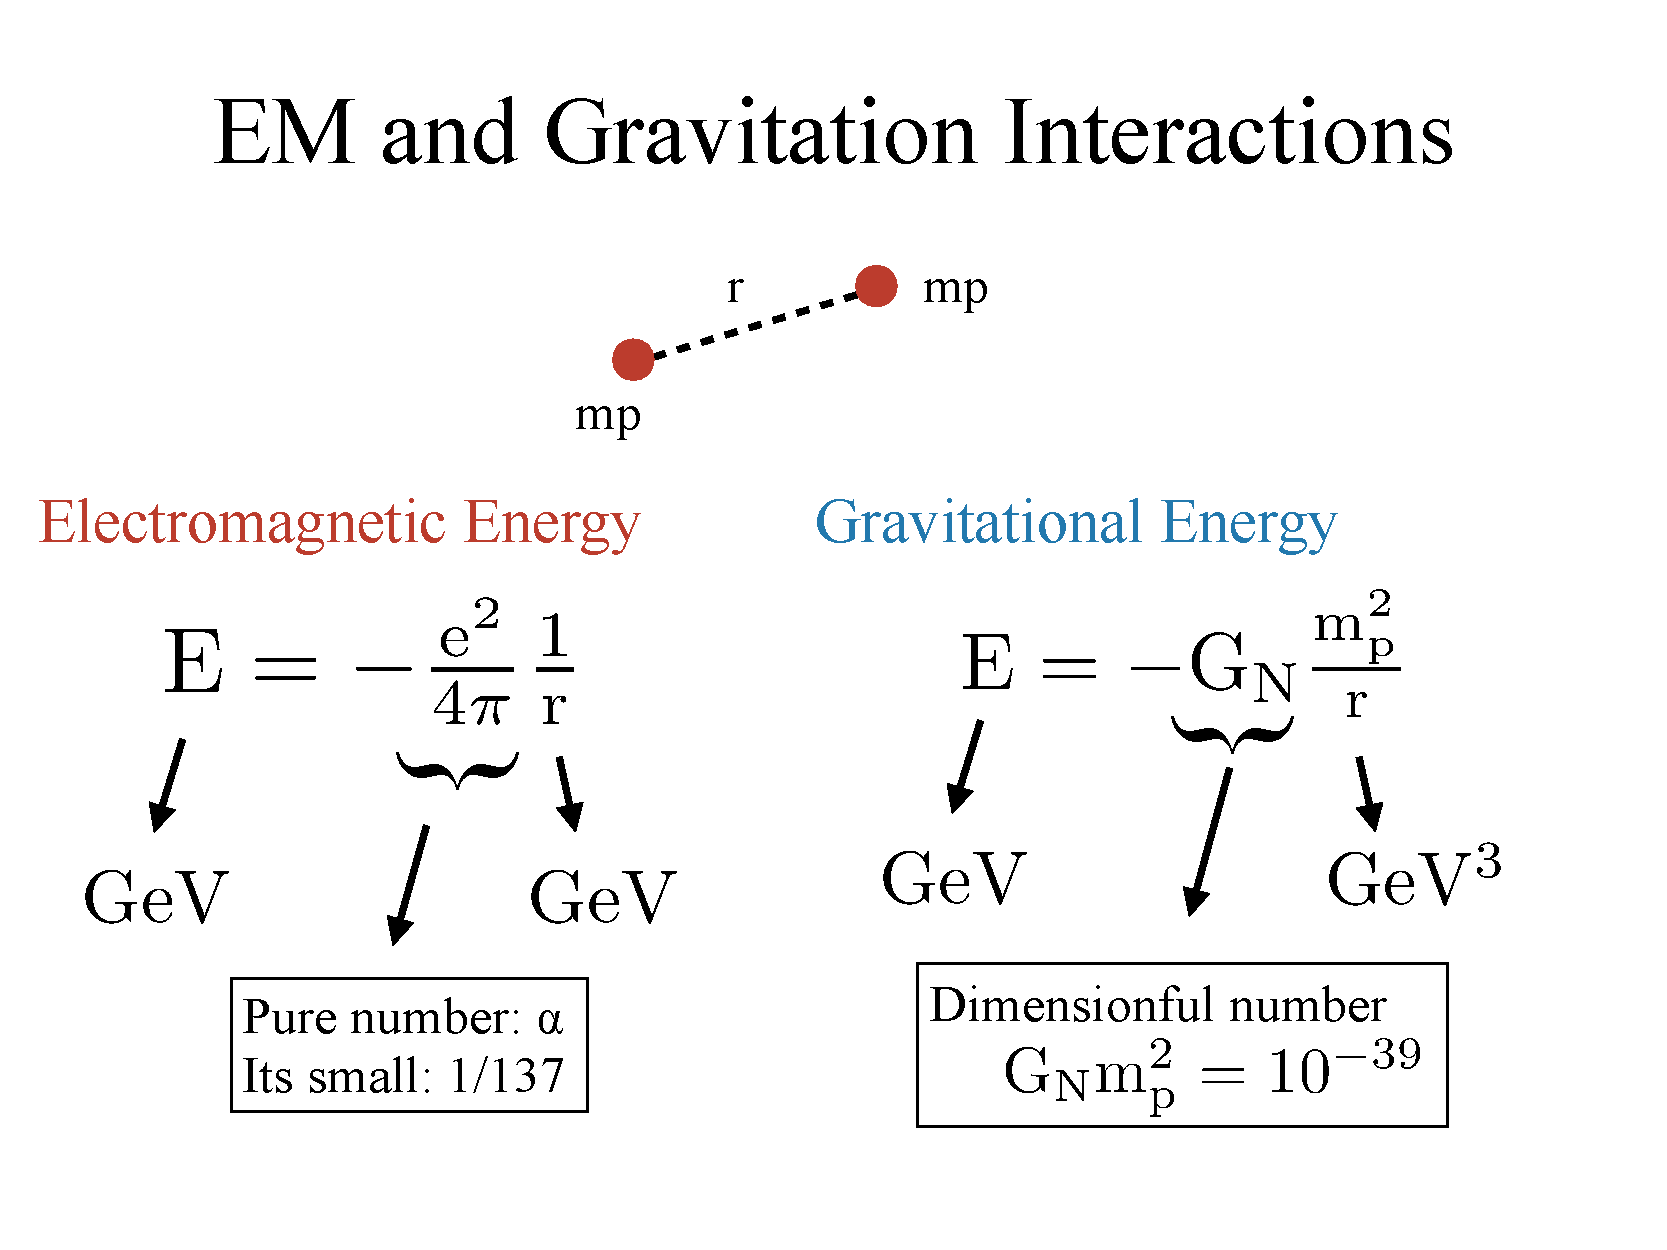
\includegraphics[width=0.9\textwidth]{./EMandGravity.pdf}
\end{figure}

\textbf{The world with 4 numbers.}\\
\underline{Claim:} $\sim$everything in world combination of these numbers\\
\begin{itemize}
\item[-]\mp = 1 GeV 
\item[-]$\alpha$ = 1/137
\item[-]\me = 10$^{-3}$ \GeV
\item[-]\aG $\equiv$ $G_N \mp^2$ = $10^{-39}$
\end{itemize}

Will work through some quick examples.

\underline{\textbf{Atoms:}}



\underline{\textbf{Solids:}}


\underline{\textbf{Planets:}}

\underline{\textbf{Life etc.:}}

Homework:
What is your major/minor ? 
When do you plan on graduating?
What do you want to do after graduation ? (eg: grad school ? if so, what subject ?)
What do you most want to get out of this course ? 

Calculate the local strength of gravity $g_{\textrm{local}}$ in terms of $\alpha$,\aG,\mp and \me.
What is your estimated value in mks units ?

Estimate an limit on the size of life.
Assume life is a solid. 

 

\end{document}


